% VLDB template version of 2020-08-03 enhances the ACM template, version 1.7.0:
% https://www.acm.org/publications/proceedings-template
% The ACM Latex guide provides further information about the ACM template

\documentclass[sigconf, nonacm]{acmart}
%% The following content must be adapted for the final version
% paper-specific
\newcommand\vldbdoi{XX.XX/XXX.XX}
\newcommand\vldbpages{XXX-XXX}
% issue-specific
\newcommand\vldbvolume{14}
\newcommand\vldbissue{1}
\newcommand\vldbyear{2020}
% should be fine as it is
\newcommand\vldbauthors{\authors}
\newcommand\vldbtitle{\shorttitle} 
% leave empty if no availability url should be set
\newcommand\vldbavailabilityurl{http://vldb.org/pvldb/format_vol14.html}
% whether page numbers should be shown or not, use 'plain' for review versions, 'empty' for camera ready
\newcommand\vldbpagestyle{plain} 

\usepackage{enumitem}
\newlist{steps}{enumerate}{1}
\setlist[steps, 1]{leftmargin=*, label =  Step \arabic*:}
\newlist{properties}{enumerate}{1}
\setlist[properties, 1]{leftmargin=*, label =  Property \arabic*:,}

\begin{document}
\title{Incremental Parallel Frequent Itemsets Mining (IPFIM) using Ordered Trees and Spark}

%%
%% The "author" command and its associated commands are used to define the authors and their affiliations.

\author{Lev Kuznetsov}
\affiliation{%
  \institution{The Open University of Israel}
  \streetaddress{P.O. Box 1212}
  \city{Raanana}
  \state{Israel}
  \postcode{43017-6221}
}
\email{lev.kuznets@gmail.com}

\author{Ehud Gudes}
\orcid{0000-0002-1825-0097}
\affiliation{%
  \institution{The Open University of Israel}
  \streetaddress{1 Th{\o}rv{\"a}ld Circle}
  \city{Raanana}
  \state{Israel}
}
\email{ehudgu@openu.ac.il}

%%
%% The abstract is a short summary of the work to be presented in the
%% article.
\begin{abstract}
The frequent itemset mining (FIM) problem has been around pretty much since the definition of the term 'data' in the previous century. Whenever there is a collection of data, one of the basic analysis we would like to perform, is finding relations within the data. One of those basic 'relations', is to find all the sets of data that appear together in an important frequency (usually greater than a predefined threshold).  The process of finding such items is called Mining, and thus the term - Frequent Itemset Mining (FIM). Frequent itemset can later reveal association rules and relations between variables. This research area in data science is applied to domains such as recommender systems (e.g. what are the set of items usually ordered together), bioinformatics (e.g. what are the genes coexpressed in a given condition), decision making, clustering, website navigation and many more.

Many algorithms were developed during time to find frequent item sets in a database, and they are mostly focused on Apriori ~\cite{agrawal1994fast} and FP-Growth~\cite{kohefficient} techniques.  The later is further discussed in section TODO.

This work focuses on using tree based structure for parallel and incremental mining. 

As the access to online resources grew, so does the size of the databases,. Today’s databases’ sizes go far beyond capabilities of a single machine. The need to provide better performance has grown and platforms for parallel computation, and the frameworks who support them, also became main stream.

 
We will elaborate more on these frameworks, specifically on Spark vs Hadoop in section [TODO].

%is an examples of such a framework and is commonly used for Big-Data processing. We will discuss more on Spark and other frameworks 

Besides the size of the databases, a growing online access also increased the need for incremental updates. 
\iffalse
In case of a slight database update, like add-on of new transactions to the DB, some algorithms require a rerun of the whole database.
With the need of better performance To provide better performance, parallel execution frameworks, such as Hadoop and Spark, become more accessible and common,  and as such, so does the adoption of classical algorithms to parallel execution.  
\fi
Such events happen with high velocity in current databases and making full recalculation may be far from optimal. 

To achieve this, the proposed algorithm is using a combination of two techniques. As a high-level overview, the PFP~\cite{li2008pfp} algorithm is the base algorithm for parallel mining and CanTree~\cite{leung2005cantree} as the base structure for incremental updates.  As the framework for computation, Spark was chosen~\cite{spark},  and will be detailed more in section [TODO]. 

\iffalse
It is important to mention that a similar approach was already developed by~\cite{song2017} at 2017, but was added as a reference after implementation and results, and we will discuss and compare to this paper in details in section [TODO]. 
\fi
In this paper we will also present a new approach for incremental group updates by using a greedy set-cover algorithm, where the motivation is to optimize groups for parallel calculations. However, as we will show from our experiments, the overhead of regrouping using hashmaps, is far larger than using random group deviation. 

The paper is divided as following: Section 2 and 3 will review related work and background, and will provide examples for the used algorithms. Section 4 and 5 will present the IPFIM algorithm, and an improvement, based on partial frequency sort and min min threshold  [TODO]. Section 6 will discuss comparison to ~\cite{song2017}.  Section 7 will present an approach for trying to optimize grouping by using greedy set-cover algorithm for optimized group mining. Section 8 will presents and discuss experimental results and section 9 will present conclusion and summarize discussion.

\end{abstract}

\maketitle

%%% do not modify the following VLDB block %%
%%% VLDB block start %%%
\pagestyle{\vldbpagestyle}
\begingroup\small\noindent\raggedright\textbf{PVLDB Reference Format:}\\
\vldbauthors. \vldbtitle. PVLDB, \vldbvolume(\vldbissue): \vldbpages, \vldbyear.\\
\href{https://doi.org/\vldbdoi}{doi:\vldbdoi}
\endgroup
\begingroup
\renewcommand\thefootnote{}\footnote{\noindent
This work is licensed under the Creative Commons BY-NC-ND 4.0 International License. Visit \url{https://creativecommons.org/licenses/by-nc-nd/4.0/} to view a copy of this license. For any use beyond those covered by this license, obtain permission by emailing \href{mailto:info@vldb.org}{info@vldb.org}. Copyright is held by the owner/author(s). Publication rights licensed to the VLDB Endowment. \\
\raggedright Proceedings of the VLDB Endowment, Vol. \vldbvolume, No. \vldbissue\ %
ISSN 2150-8097. \\
\href{https://doi.org/\vldbdoi}{doi:\vldbdoi} \\
}\addtocounter{footnote}{-1}\endgroup
%%% VLDB block end %%%

%%% do not modify the following VLDB block %%
%%% VLDB block start %%%
\ifdefempty{\vldbavailabilityurl}{}{
\vspace{.3cm}
\begingroup\small\noindent\raggedright\textbf{PVLDB Artifact Availability:}\\
The source code, data, and/or other artifacts have been made available at \url{\vldbavailabilityurl}.
\endgroup
}
%%% VLDB block end %%%

\chapter{Introduction}
\addhtoc{chapter}{מבוא}
\label{chap:intro}

\chapter{Introduction}
\addhtoc{chapter}{מבוא}
\label{chap:intro}

\chapter{Introduction}
\addhtoc{chapter}{מבוא}
\label{chap:intro}

\input{includes/introduction}




\section{PRELIMINARY AND RELATED WORK}

This paper will focus on the use case of an incremental mining, such as streaming data, while reading the full DB only once.

\begin{figure}
  \centering
  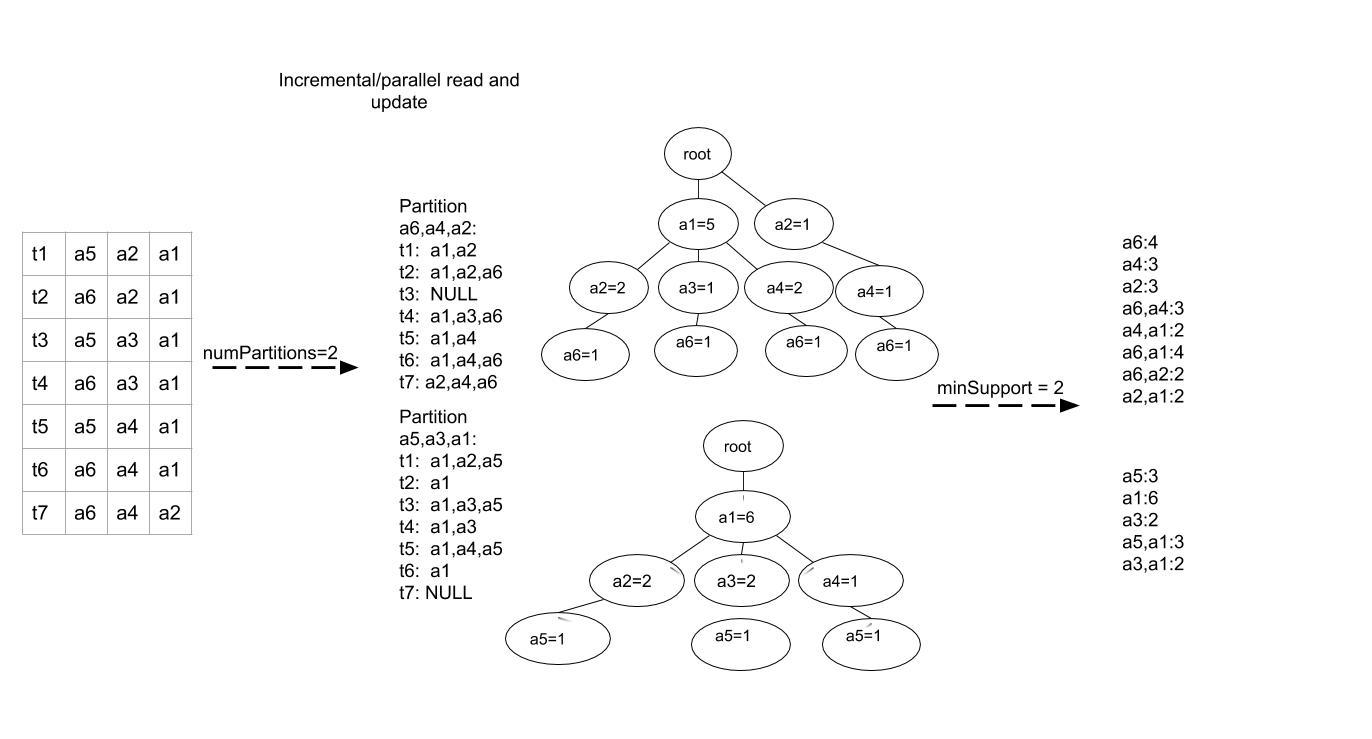
\includegraphics[width=\linewidth]{figures/IncrementalTreeMining}
  \caption{An example of trees and mining for minSup=2 and 2 partitions}
  \label{fig:incrementalParallelMining}
\end{figure}

\subsection{Related Work}
  One of the most well known algorithms for mining association rules is the Apriori algorithm~\cite{agrawal1994fast}. This algorithm is iteratively generating candidates and pruning items with low support at each step. If an item of length N is frequent, then all sub patterns must be frequent as well. Using that idea, an early prune of non-frequent itemsets removes many unnecessary candidates in later iterations.

In the year 2000, a tree based solution was introduced, FPGrowth algorithm and structure~\cite{agrawal1994fast}. This algorithm removes the need for candidate generation and yields better performance~\cite{hunyadi2011performance}. A small example is provided in \autoref{fig:fpgrowthexample}


\subsection{Incremental Frequent Itemsets Mining}
Incremental updates is to recompute outputs which depend on the incoming inputs only, without recomputing the whole data.

The basic challenge in incremental updates for frequent items mining, is a non consistent frequency order. Several algorithms such as AFPIM~\cite{koh2004efficient}, EFPIM~\cite{li2006fast} and FUFP-tree~\cite{hong2008incrementally} are keeping an updated frequency based trees, by reordering branches where frequency has changed.

The work of~\cite{leung2005cantree} presented a Canonical Tree (CanTree) which preserves the frequency descending structure as in FP Growth mining, by relying on a predefined order, which will not affect the tree structure and correctness.

	The work of~\cite{tanbeer2009efficient} proposes an improvement to CanTree, called CompactPattern-Tree, and discusses the memory and computation limitations of CanTree for large incremental Databases. The issues are caused due to un-efficient tree structure, and CP-Tree is proposing an improvement by periodically (using a proposed guideline) updating the order of the construction literals list (l-list) and rebuilding the trees. As mention in the original article and as seen by our experiments, the CanTree and CP-Tree has a similar tree size, and the difference for our test cases was 10\% in tree sizes. However as seen in our results, using semi-frequency based order, improves the mining results by 10X and more for smaller minSupport values.
	
	

\subsection{Parallel Frequent Itemsets mining}
The difficulty in parallelizing FP-growth is to distribute iterations to parallel trees while still allowing correct mining. PFP~\cite{li2008pfp} is solving this by dividing the DB transactions to independent trees using a Group-List, where every group consists of items, and redistributing iterations in the DB based on this list.
PFP~\cite{li2008pfp} is working in the following steps:

\begin{steps}
	\item Find global frequency list, F-List
	\item Group items G-list
	\item PFP:
		\begin{enumerate}
			\item For each Ti, order by F-List frequency
			\item For each aj in Ti, replace aj with gi that aj belongs to its group
			\item For each gi, if it appears in Ti, find its right-most location in Ti, say L and output:
 <key'=gi; value'={Ti[0]…Ti[L]}>
 			\item Group by key' = gi
 			\item For each group gi, build appropriate tree
 			\item For each group gi, mine the generated tree (filter items not in gi).
		\end{enumerate}
\end{steps}

\begin{figure}
  \centering
  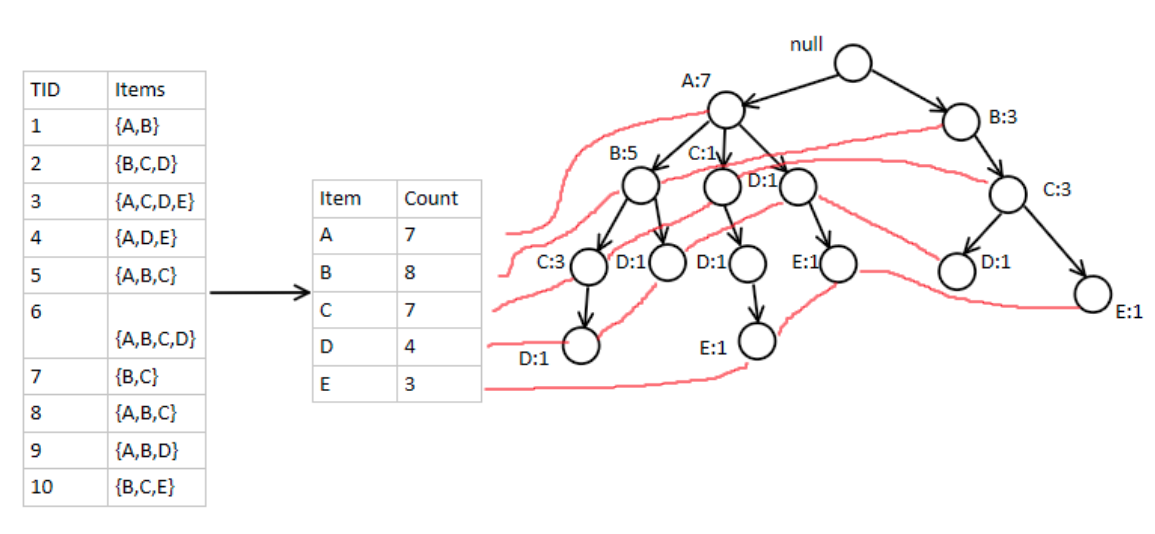
\includegraphics[width=\linewidth]{figures/fpgrowthexample}
  \caption{FPGrowth example}
  \label{fig:fpgrowthexample}
\end{figure}

It is important to mention that there might be some duplicates at several groups of frequent itemsets in stage 3.6, but this is solved when filtering the 1-length items that are not relevant to the specific group. This duplication also affects the size of the generated trees and overall memory.

\subsection{Incremental and Parallel Frequent itemsets mining}

Combining the previous 2 sections, yields an algorithm that does not rely on frequency order and uses parallelism advantages for computations of FIS.
The drawbacks are also drawn from the 2 algorithms - large memory consumption for saving all items and recursively calculating FIS. As we will show later in the \hyperref[sec:improvements]{Improvments} section, using an approach similar to ~\cite{kohefficient} and maintaining a pre-min support, together with using a semi-freq-order as in ~\cite{tanbeer2009efficient}, will significantly improve memory and mining runtime results.



\chapter{Background And Related Work}
\chapter{Background And Related Work}
\chapter{Background And Related Work}
\input{includes/background}
\input{includes/relatedwork}
%\addhtoc{chapter}{רקע}
\label{chap:background}
\
\section{PRELIMINARY AND RELATED WORK}

This paper will focus on the use case of an incremental mining, such as streaming data, while reading the full DB only once.

\begin{figure}
  \centering
  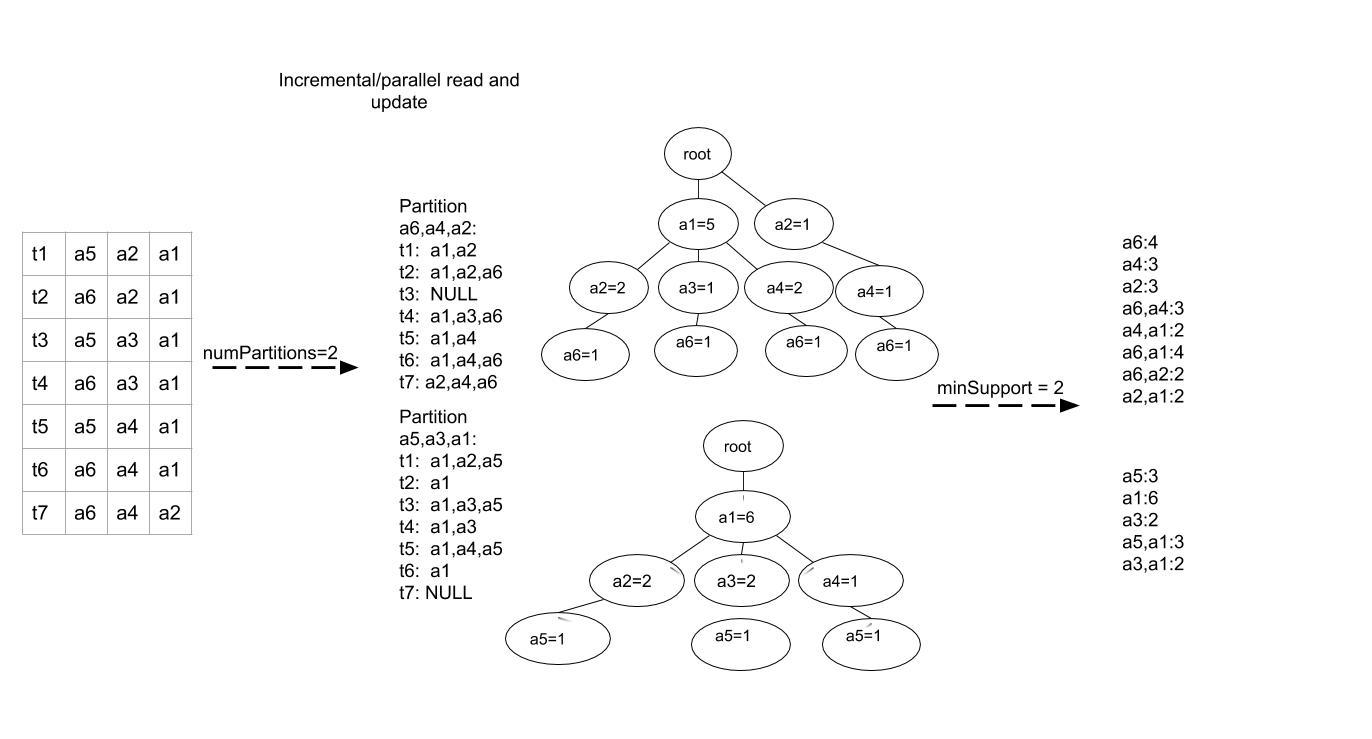
\includegraphics[width=\linewidth]{figures/IncrementalTreeMining}
  \caption{An example of trees and mining for minSup=2 and 2 partitions}
  \label{fig:incrementalParallelMining}
\end{figure}

\subsection{Related Work}
  One of the most well known algorithms for mining association rules is the Apriori algorithm~\cite{agrawal1994fast}. This algorithm is iteratively generating candidates and pruning items with low support at each step. If an item of length N is frequent, then all sub patterns must be frequent as well. Using that idea, an early prune of non-frequent itemsets removes many unnecessary candidates in later iterations.

In the year 2000, a tree based solution was introduced, FPGrowth algorithm and structure~\cite{agrawal1994fast}. This algorithm removes the need for candidate generation and yields better performance~\cite{hunyadi2011performance}. A small example is provided in \autoref{fig:fpgrowthexample}


\subsection{Incremental Frequent Itemsets Mining}
Incremental updates is to recompute outputs which depend on the incoming inputs only, without recomputing the whole data.

The basic challenge in incremental updates for frequent items mining, is a non consistent frequency order. Several algorithms such as AFPIM~\cite{koh2004efficient}, EFPIM~\cite{li2006fast} and FUFP-tree~\cite{hong2008incrementally} are keeping an updated frequency based trees, by reordering branches where frequency has changed.

The work of~\cite{leung2005cantree} presented a Canonical Tree (CanTree) which preserves the frequency descending structure as in FP Growth mining, by relying on a predefined order, which will not affect the tree structure and correctness.

	The work of~\cite{tanbeer2009efficient} proposes an improvement to CanTree, called CompactPattern-Tree, and discusses the memory and computation limitations of CanTree for large incremental Databases. The issues are caused due to un-efficient tree structure, and CP-Tree is proposing an improvement by periodically (using a proposed guideline) updating the order of the construction literals list (l-list) and rebuilding the trees. As mention in the original article and as seen by our experiments, the CanTree and CP-Tree has a similar tree size, and the difference for our test cases was 10\% in tree sizes. However as seen in our results, using semi-frequency based order, improves the mining results by 10X and more for smaller minSupport values.
	
	

\subsection{Parallel Frequent Itemsets mining}
The difficulty in parallelizing FP-growth is to distribute iterations to parallel trees while still allowing correct mining. PFP~\cite{li2008pfp} is solving this by dividing the DB transactions to independent trees using a Group-List, where every group consists of items, and redistributing iterations in the DB based on this list.
PFP~\cite{li2008pfp} is working in the following steps:

\begin{steps}
	\item Find global frequency list, F-List
	\item Group items G-list
	\item PFP:
		\begin{enumerate}
			\item For each Ti, order by F-List frequency
			\item For each aj in Ti, replace aj with gi that aj belongs to its group
			\item For each gi, if it appears in Ti, find its right-most location in Ti, say L and output:
 <key'=gi; value'={Ti[0]…Ti[L]}>
 			\item Group by key' = gi
 			\item For each group gi, build appropriate tree
 			\item For each group gi, mine the generated tree (filter items not in gi).
		\end{enumerate}
\end{steps}

\begin{figure}
  \centering
  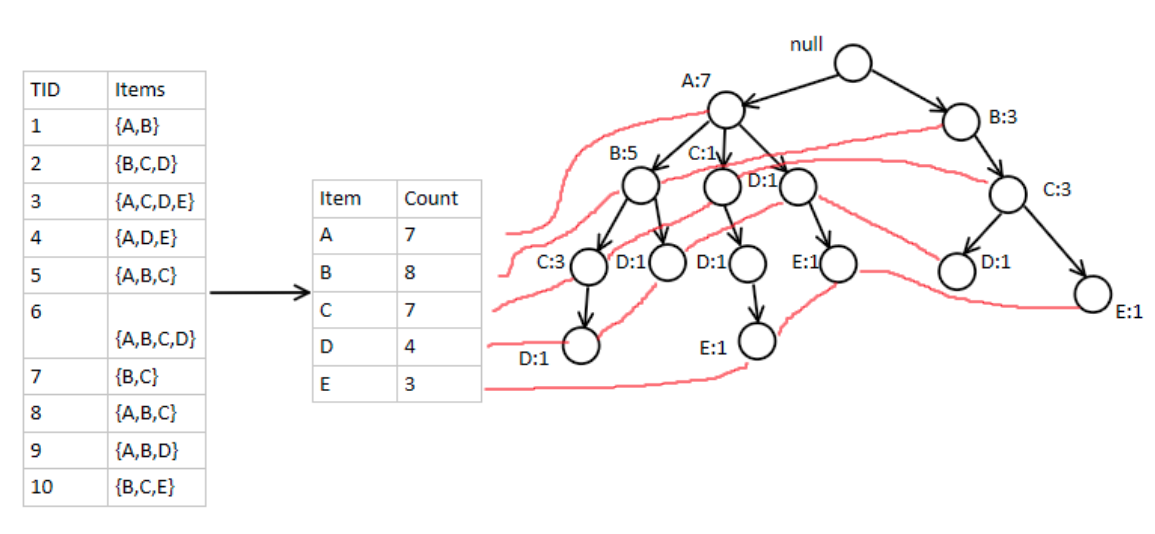
\includegraphics[width=\linewidth]{figures/fpgrowthexample}
  \caption{FPGrowth example}
  \label{fig:fpgrowthexample}
\end{figure}

It is important to mention that there might be some duplicates at several groups of frequent itemsets in stage 3.6, but this is solved when filtering the 1-length items that are not relevant to the specific group. This duplication also affects the size of the generated trees and overall memory.

\subsection{Incremental and Parallel Frequent itemsets mining}

Combining the previous 2 sections, yields an algorithm that does not rely on frequency order and uses parallelism advantages for computations of FIS.
The drawbacks are also drawn from the 2 algorithms - large memory consumption for saving all items and recursively calculating FIS. As we will show later in the \hyperref[sec:improvements]{Improvments} section, using an approach similar to ~\cite{kohefficient} and maintaining a pre-min support, together with using a semi-freq-order as in ~\cite{tanbeer2009efficient}, will significantly improve memory and mining runtime results.


%\addhtoc{chapter}{רקע}
\label{chap:background}
\
\section{PRELIMINARY AND RELATED WORK}

This paper will focus on the use case of an incremental mining, such as streaming data, while reading the full DB only once.

\begin{figure}
  \centering
  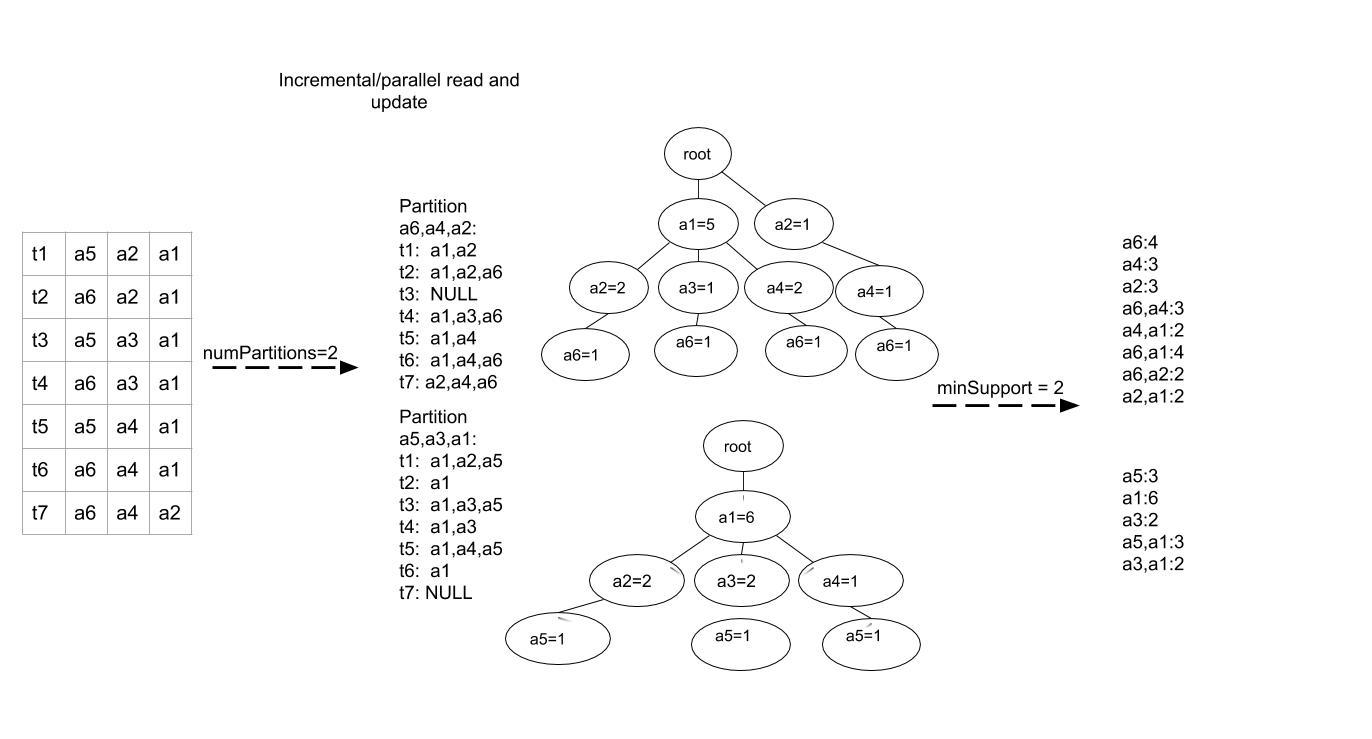
\includegraphics[width=\linewidth]{figures/IncrementalTreeMining}
  \caption{An example of trees and mining for minSup=2 and 2 partitions}
  \label{fig:incrementalParallelMining}
\end{figure}

\subsection{Related Work}
  One of the most well known algorithms for mining association rules is the Apriori algorithm~\cite{agrawal1994fast}. This algorithm is iteratively generating candidates and pruning items with low support at each step. If an item of length N is frequent, then all sub patterns must be frequent as well. Using that idea, an early prune of non-frequent itemsets removes many unnecessary candidates in later iterations.

In the year 2000, a tree based solution was introduced, FPGrowth algorithm and structure~\cite{agrawal1994fast}. This algorithm removes the need for candidate generation and yields better performance~\cite{hunyadi2011performance}. A small example is provided in \autoref{fig:fpgrowthexample}


\subsection{Incremental Frequent Itemsets Mining}
Incremental updates is to recompute outputs which depend on the incoming inputs only, without recomputing the whole data.

The basic challenge in incremental updates for frequent items mining, is a non consistent frequency order. Several algorithms such as AFPIM~\cite{koh2004efficient}, EFPIM~\cite{li2006fast} and FUFP-tree~\cite{hong2008incrementally} are keeping an updated frequency based trees, by reordering branches where frequency has changed.

The work of~\cite{leung2005cantree} presented a Canonical Tree (CanTree) which preserves the frequency descending structure as in FP Growth mining, by relying on a predefined order, which will not affect the tree structure and correctness.

	The work of~\cite{tanbeer2009efficient} proposes an improvement to CanTree, called CompactPattern-Tree, and discusses the memory and computation limitations of CanTree for large incremental Databases. The issues are caused due to un-efficient tree structure, and CP-Tree is proposing an improvement by periodically (using a proposed guideline) updating the order of the construction literals list (l-list) and rebuilding the trees. As mention in the original article and as seen by our experiments, the CanTree and CP-Tree has a similar tree size, and the difference for our test cases was 10\% in tree sizes. However as seen in our results, using semi-frequency based order, improves the mining results by 10X and more for smaller minSupport values.
	
	

\subsection{Parallel Frequent Itemsets mining}
The difficulty in parallelizing FP-growth is to distribute iterations to parallel trees while still allowing correct mining. PFP~\cite{li2008pfp} is solving this by dividing the DB transactions to independent trees using a Group-List, where every group consists of items, and redistributing iterations in the DB based on this list.
PFP~\cite{li2008pfp} is working in the following steps:

\begin{steps}
	\item Find global frequency list, F-List
	\item Group items G-list
	\item PFP:
		\begin{enumerate}
			\item For each Ti, order by F-List frequency
			\item For each aj in Ti, replace aj with gi that aj belongs to its group
			\item For each gi, if it appears in Ti, find its right-most location in Ti, say L and output:
 <key'=gi; value'={Ti[0]…Ti[L]}>
 			\item Group by key' = gi
 			\item For each group gi, build appropriate tree
 			\item For each group gi, mine the generated tree (filter items not in gi).
		\end{enumerate}
\end{steps}

\begin{figure}
  \centering
  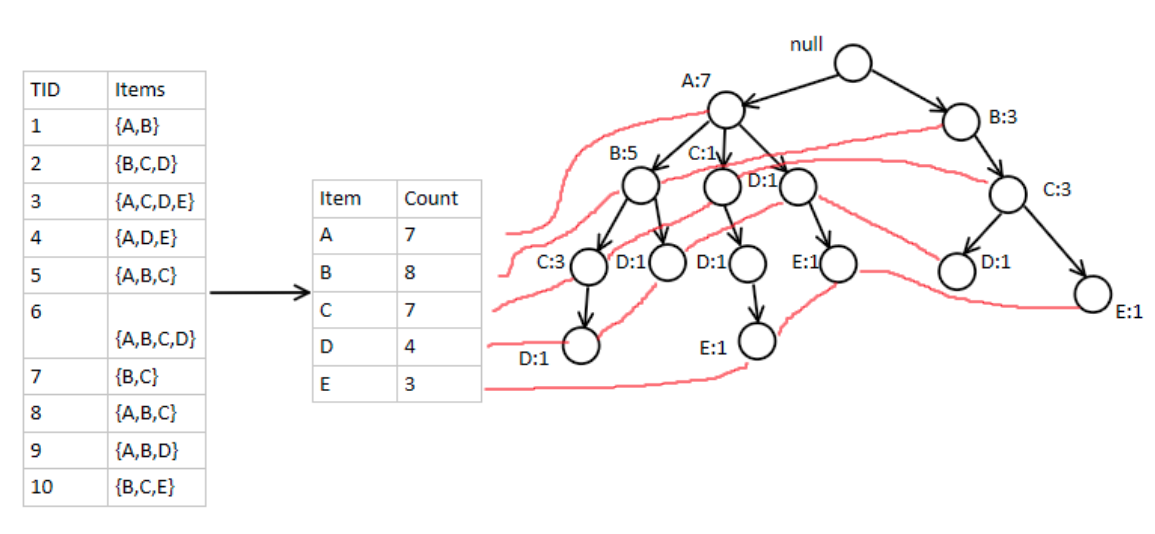
\includegraphics[width=\linewidth]{figures/fpgrowthexample}
  \caption{FPGrowth example}
  \label{fig:fpgrowthexample}
\end{figure}

It is important to mention that there might be some duplicates at several groups of frequent itemsets in stage 3.6, but this is solved when filtering the 1-length items that are not relevant to the specific group. This duplication also affects the size of the generated trees and overall memory.

\subsection{Incremental and Parallel Frequent itemsets mining}

Combining the previous 2 sections, yields an algorithm that does not rely on frequency order and uses parallelism advantages for computations of FIS.
The drawbacks are also drawn from the 2 algorithms - large memory consumption for saving all items and recursively calculating FIS. As we will show later in the \hyperref[sec:improvements]{Improvments} section, using an approach similar to ~\cite{kohefficient} and maintaining a pre-min support, together with using a semi-freq-order as in ~\cite{tanbeer2009efficient}, will significantly improve memory and mining runtime results.


%\addhtoc{chapter}{רקע}
\label{chap:background}
\

\section{IPFIM - Incremental Parallel Frequent Itemsets Mining}
\label{sec:ipfim}
The implementation of this algorithm strongly depends on PFP~\cite{li2008pfp}. To support incremental tree updates, we are using a predefined comparison function to arrange the items insertion order, as used in CanTree~\cite{leung2005cantree}.

\subsection{IPFIM Outline}
The combination of the previously mentioned algorithms will provide an incremental and parallel algorithm for mining FIS.  The highlevel algorithm is presented in ~\ref{alg:ipfim}, while the inner update of every iteration is in ~\ref{alg:ipfimiteration}.

\begin{algorithm}
  \caption{IPFIM}
  \begin{algorithmic}[1]
   \label{alg:ipfim}
    \Procedure{IPFIM}{minSupport, iterationsArray[],numIterations, sortFunction,partitioner}
    \State $canTrees\gets$ RDD[$|partitioner|$] of empty $CanTree$ objects
    \State $fisArray\gets$ array[$numIterations$]
    \For{$i\gets 0\ ;\  i\! <\! numIterations \ ;\  i\! +\! +$}
    	\State $canTrees \gets IPFIMIteration(iterationsArray[i],canTrees,sortFunction,partitioner)$
    	\State $fisArray[i] \gets mineCanTrees(canTrees,minSupport)$ \Comment{Same as in FPGrowth}
    \EndFor
    \State \textbf{return} $fisArray$
    \EndProcedure
  \end{algorithmic}
\end{algorithm}

\begin{algorithm}
  \caption{IPFIMIteration}
  \begin{algorithmic}[1]
   \label{alg:ipfimiteration}
    \Procedure{IPFIMIteration}{data,canTrees,sortFunction,partitioner}
    \State $sortedTransactions\gets\text{order data by sortFunction}$
    \State $partitionedTransactions\gets\text{map sortedTransactions to key'=g; value'={t\textsubscript{i}[0]…t\textsubscript{i}[L]}}$ \Comment{As in PFP}
	\State $canTrees \gets\text{Reduce partitionedTransactions and update trees}$
	\State \textbf{return} $canTrees$
    \EndProcedure
  \end{algorithmic}
\end{algorithm}

For every iteration there the following map/reduce jobs:
\begin{enumerate}
\item Map: Read and sort data
\item Map: Split based on the partitioner
\item Reduce: Add to proper CanTree object in group
\end{enumerate}
Followed by the mining map:
\begin{enumerate}
\item Map: every partition, 1-length fis to its projected recursive tree, and output FIS
\end{enumerate}

\subsubsection{IPFIM Example}
 \autoref{fig:IPFIMexample} shows an example for a 2 partition calculation of CanTrees based on the partition function of $\{a6,a4,a2\}\to 0$ and $\{a5,a3,a1\}\to 1$.
\begin{figure}
  \centering
  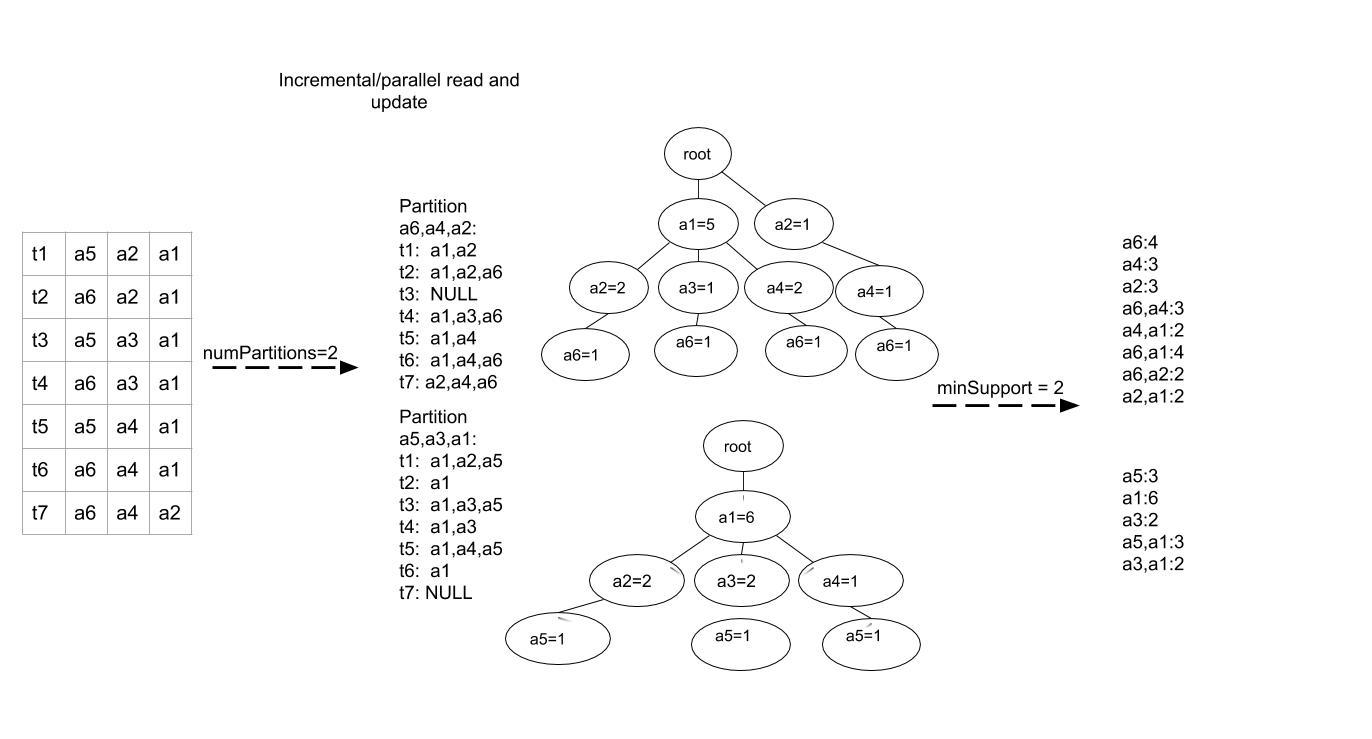
\includegraphics[width=\linewidth]{figures/IncrementalTreeMining1}
  \caption{IPFIM example}
  \label{fig:IPFIMexample}
\end{figure}

%The highlevel steps for the combined algorithm are:
%\begin{steps}
%	\item Define a comparison function: compare(item1,item2)->bool
%	\item Define a Partition function: partition(item)->Long
%	\item For every increment:
%		\begin{enumerate}
%		\label{sec:ipfimAlg}
%			\item PFP: Scan transaction and sort using compare function
%			\item PFP: Scan sorted transactions and replace using the PFP \autoref{alg:pfpalg} lines 7:9
%			\label{sec:ipfimpf}
%			\item PFP+CanTree: Update each group partition with the transactions of the group and
%			 update the CanTree (save the partial CanTree)
%			\item PFP: Run FP-Growth on every partitions CanTree and reduce results for final output
%		\end{enumerate}
%\end{steps}


\subsection{Correctness}
The correctness of IPFIM comes directly from the correctness of the 2 combined algorithms. 
The proof is pretty simple by using contradiction: 
\begin{enumerate}
	\item Assuming that the following item-set of length k,  \{t\textsubscript{i},... ,t\textsubscript{i+k-1}\}, became frequent at iteration l, from transaction T\textsubscript{j}, but was not part of the reported output.
	\item According to \autoref{sec:ipfimpf}, transaction T\textsubscript{j} is translated to <key'=g; value'={t\textsubscript[0]…t\textsubscript[k]}> and added to the CanTree of partition g.
	\item If it was not added at this point, PFP is not correct, false $\blacksquare $
	\item Otherwise it was added to the CanTree, but was not mined. CanTree is not correct, false $\blacksquare $. 
\end{enumerate}

Similar method is used as a proof of the other use cases - a false frequent itemset, a frequent itemset is no longer frequent etc.


\chapter{Experiments Results }
%\addhtoc{chapter}
%{נושא1}
\label{chap:results}

\chapter{Experiments Results }
%\addhtoc{chapter}
%{נושא1}
\label{chap:results}

\chapter{Experiments Results }
%\addhtoc{chapter}
%{נושא1}
\label{chap:results}

\input{includes/results}


%\begin{theorem}
%Your theorem here.
%\end{theorem}
%\textbf{Proof:}
%Your proof here
%\QEDA

%\subsection{subsection1}
%\addhtoc{subsection}{תת-סעיף 1}




%\begin{theorem}
%Your theorem here.
%\end{theorem}
%\textbf{Proof:}
%Your proof here
%\QEDA

%\subsection{subsection1}
%\addhtoc{subsection}{תת-סעיף 1}




%\begin{theorem}
%Your theorem here.
%\end{theorem}
%\textbf{Proof:}
%Your proof here
%\QEDA

%\subsection{subsection1}
%\addhtoc{subsection}{תת-סעיף 1}




\section{Improvements - Need to add SetCover results and explanations}
\label{sec:improvements}

While developing and testing the algorithm, 2 main obstacles prevented from using larger datasets and smaller minSupport:
\begin{enumerate}
	\item Memory - Tree size.
	\item Computation Time - Tree order.
\end{enumerate}

To handle these obstacles, 2 techniques were implemented.
To handle the computation time, an approach similar to CPTree~\cite{tanbeer2009efficient} was tested, where we defined a semi-frequency order on 1st dataset half, and used it for the rest of the iterations. New items were sorted canonically.

To handle the memory limitation, which is caused by the construction of a large tree, a partial approach of AFPIM~\cite{koh2004efficient} was implemented. We added a pre-min support to identify pre-frequent items. For the simplicity of the experiment, items which where not frequent in iteration i, and will become frequent after sum of j iterations, are waived. A trade-off between missing items and tree size can be controlled using the pre-min parameter. 

\subsection{IPFIM Improved vs IPFIM - Computation}
Although the size of the tree was not effected by more than 10\%, when using semi-frequency order, computation time was improved by ~30X when running single partition, as seen in \autoref{fig:partialcannonical}.
\begin{figure}
  \centering
  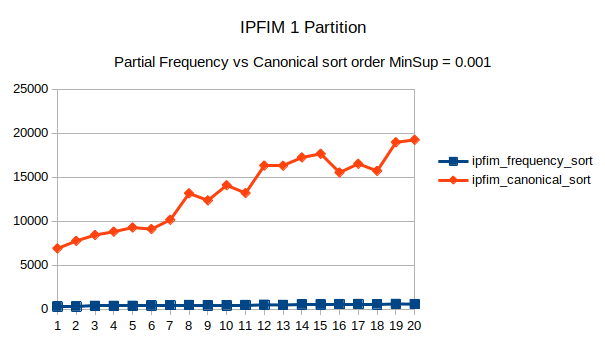
\includegraphics[width=\linewidth]{figures/ipfim_freq_vs_can_sort}
  \caption{IPFIM partial frequency sort vs IPFIM cannonical sort}
  \label{fig:partialcannonical}
\end{figure}

\subsection{IPFIM Improved vs IPFIM - Memory}
Using a partial approach of AFPIM~\cite{koh2004efficient}, we were able to run synthetic datasets of 100M transactions and 100k unique item sets. The results, compared to PFP, for 100 partitions, min support of 0.01 and 0.003 can be seen  in \autoref{fig:ipfimImpT20}. As there is only 1 dataset scan for IPFIM, and we pre-defined the semi-frequency order, the results are 10x faster even for 1st iteration, and improve to 25x for last one.

\begin{figure}
  \centering
  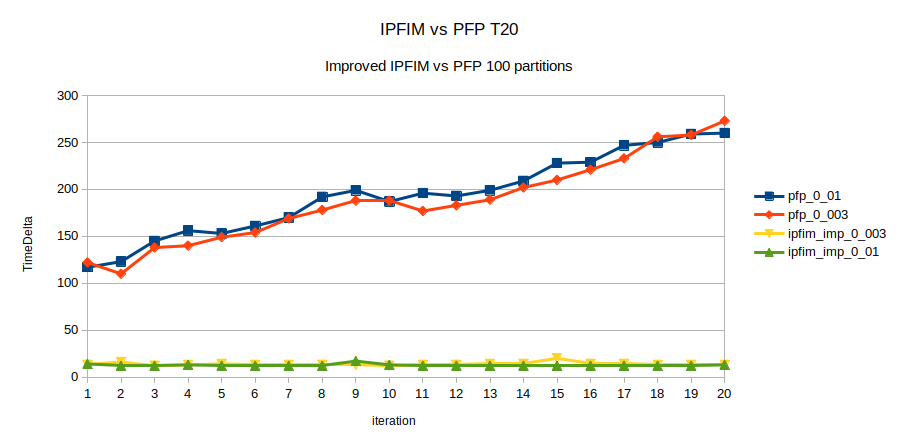
\includegraphics[width=\linewidth]{figures/t20_ipfim_imp_vs_pfp}
  \caption{IPFIM pre-min, semi-frequency vs PFP}
  \label{fig:ipfimImpT20}
\end{figure}


\section{Conclusions}
For a single computation of frequent items, the benchmark for performance and memory for IPFIM, is PFP. This is because IPFIM is using similar techniques, and FP tree is the optimal structure for this purpose (except some variations mentioned in previous sections, e.g. optimal sharding).
As already mentioned in the \hyperref[sec:discussion]{\textit{discussion}} section, when there is a relatively equal ratio between reading a dataset and computation time of frequent item sets, IPFIM with the suggested improvements out performs PFP. However, for large FIS computation time, this advantage is negligible in total.

Using a canonical order approach, as in Cantree, was almost not practical for large data sets, nor for small min support calculations. The improvement of using a semi-frequency and pre-min support limitation, provides the best balance , and provides best performance.

For future work, it is interesting to enhance PFP to use "smart" grouping. For example trying to use greedy set cover to find groups for of frequent itemsets.


\begin{acks}

% This work was supported by the [...] Research Fund of [...] (Number [...]). Additional funding was provided by [...] and [...]. We also thank [...] for contributing [...].

I would like to thank Prof. Gudes, my instructor, for his time and guidance in making this thesis.  I would also use this acknowledgement to thanks The Open University of Israel for providing the opportunity to ...
And last but certainly not least, I would like to thank my family and my wife Jenny for supporting me during that time.

\end{acks}

%\clearpage

\bibliographystyle{ACM-Reference-Format}
\bibliography{sample}

\end{document}
\endinput
